\documentclass{article}
%\usepackage{expl3}
%\usepackage{tikz}
\usepackage{pgfplots}
%\usepackage{tagpdf}
%\usepackage{fancyhdr}
%\usepackage{xparse}
%\usepackage{etoolbox}
\usepackage{accessibility}
%\usepackage{indentfirst}


\pgfplotsset{compat=1.16}

\title{This is My Title}


\begin{document}

\tableofcontents

\newpage

\section{TikzPicture}



%\tagstructbegin{tag=Document}
%\begin{figure}
\begin{accfigure}{ALT TEXT}[h]
%\tagstructbegin{tag=Figure, alttext=ALT TEXT GOES HERE}
%\tagmcbegin{tag=Figure}
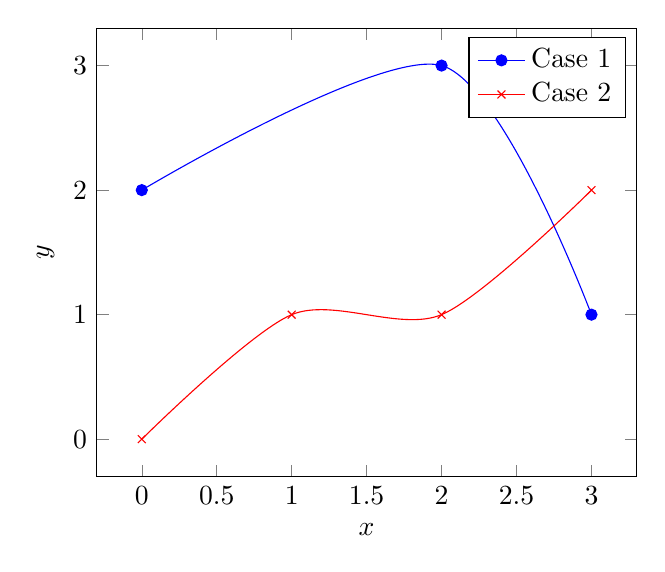
\begin{tikzpicture}
    \begin{axis}[
        xlabel=$x$,
        ylabel=$y$]
    \addplot[smooth,mark=*,blue] plot coordinates {
        (0,2)
        (2,3)
        (3,1)
    };
    \addlegendentry{Case 1}

    \addplot[smooth,color=red,mark=x]
        plot coordinates {
            (0,0)
            (1,1)
            (2,1)
            (3,2)
        };
    \addlegendentry{Case 2}
    \end{axis}
    \end{tikzpicture}

    \caption{Caption goes here}
%\tagmcend
%\end{figure}
\end{accfigure}
%\tagstructend

\subsection{Here is a Subsection}

%\tagmcbegin{tag=P}
\OpenStructMc{P}
tag! jiffy infinity affine
\CloseStructMc
%\tagmcend
%\tagstructend

\begin{accfigure}{This figure does not have a caption}[h]
%\tagstructbegin{tag=Figure, alttext=ALT TEXT GOES HERE}
%\tagmcbegin{tag=Figure}
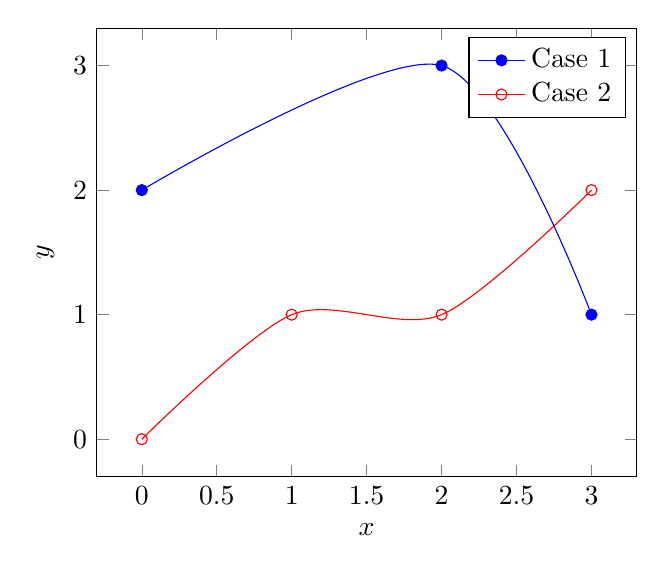
\begin{tikzpicture}
    \begin{axis}[
        xlabel=$x$,
        ylabel=$y$]
    \addplot[smooth,mark=*,blue] plot coordinates {
        (0,2)
        (2,3)
        (3,1)
    };
    \addlegendentry{Case 1}

    \addplot[smooth,color=red,mark=o]
        plot coordinates {
            (0,0)
            (1,1)
            (2,1)
            (3,2)
        };
    \addlegendentry{Case 2}
    \end{axis}
    \end{tikzpicture}

%    \caption{Caption goes here}
%\tagmcend
%\end{figure}
\end{accfigure}

\newpage

\section[Short Title]{A Section with Text Only}

\OpenStructMc{P}
Here is one paragraph. It has a bunch of sentences. It unfortunately cannot cross a page barrier. If it does, it needs to be separated into multiple `P' tags.
\CloseStructMc{}

\OpenStructMc{P}
And an even shorter paragraph here.
\CloseStructMc

\section*{A section not in the Table of Contents}

\OpenStructMc{Formula}[alttext=An example formula]
\begin{equation} \textstyle
  \mathcal{L}_{\mathcal{T}}(\vec{\lambda}) = \sum_{\mathbf{x},\mathbf{s}\in\mathcal{T}} \log P(\mathbf{x}|\mathbf{S}) - \sum_{i=1}^m \frac{\lambda_i^2}{2\sigma^2}
\end{equation}
\CloseStructMc

%\tagstructend

%\ExplSyntaxOn
%
%\__acc_open_section:n {1}
%
%\__acc_open_section:n {2}
%
%\__acc_open_section:n {2}
%
%\__acc_open_section:n {3}
%
%\__acc_open_section:n {1}
%
%\ExplSyntaxOff


\end{document} 